% generated by gen_pipe_fig.py -- do not edit by hand
\documentclass[10pt]{standalone}
\usepackage{helvet}
\renewcommand{\familydefault}{\sfdefault}
\usepackage{amsmath,amssymb}
\usepackage{tikz}
\usetikzlibrary{arrows.meta,patterns,decorations.pathmorphing}
\definecolor{cctrl}{HTML}{D6E0EC}
\definecolor{cctrlb}{HTML}{3B5675}
\definecolor{cfpu}{HTML}{FFE9A8}
\definecolor{cfpub}{HTML}{BF9000}
\definecolor{cme}{HTML}{FBE5D6}
\definecolor{cmeb}{HTML}{C55A11}
\definecolor{cl1}{HTML}{F4B183}
\definecolor{cddr}{HTML}{EAD1DC}
\definecolor{cddrb}{HTML}{8E5572}
\definecolor{cwb}{HTML}{D9EAD3}
\definecolor{cwbb}{HTML}{548235}
\newcommand{\fs}{\fontsize{6.4}{7.4}\selectfont}
\newcommand{\fss}{\fontsize{5.6}{6.4}\selectfont}
\begin{document}
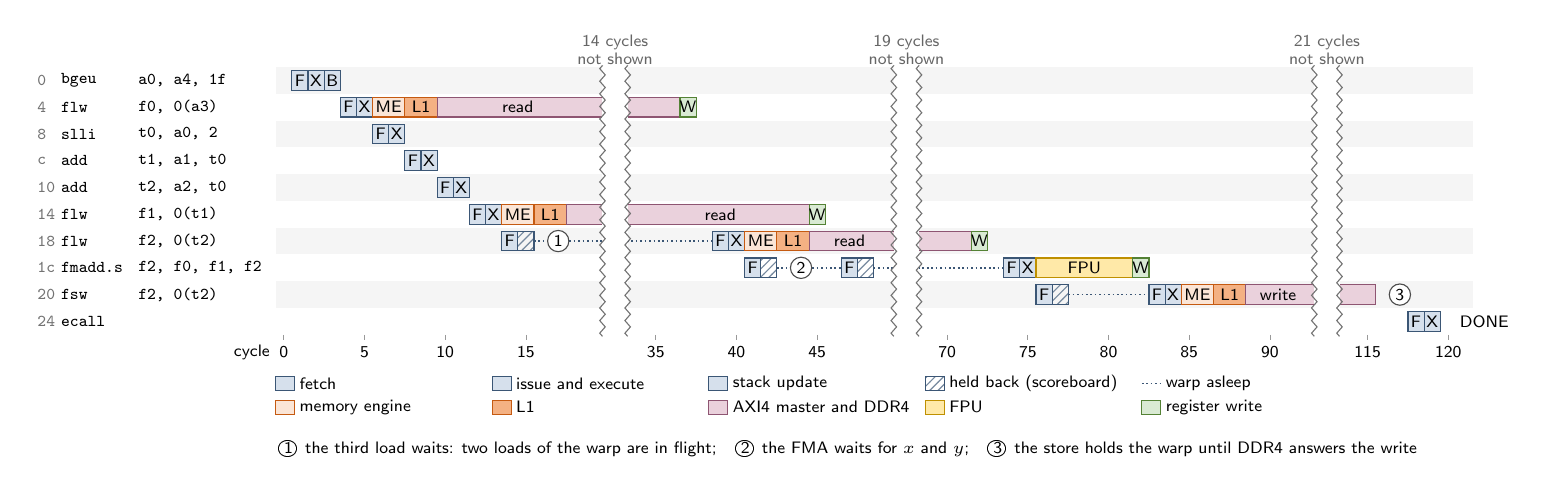
\begin{tikzpicture}[x=1cm, y=1cm,
  seg/.style={line width=0.4pt, inner sep=0pt},
  lbl/.style={font=\fs, inner sep=0.5pt},
  note/.style={font=\fss, inner sep=0.5pt, align=left},
  code/.style={font=\fss\ttfamily, inner sep=0.5pt, anchor=west},
  panel/.style={draw=none, fill=none},
  arr/.style={-{Latex[length=1.2mm, width=0.9mm]}, line width=0.45pt}]

\draw[panel] (-0.10,-1.62) rectangle (18.800,3.900);
\fill[black!4] (3.050,3.060) rectangle (18.250,3.400);
\node[code, text=black!55] at (0.0,3.230) {0};
\node[code] at (0.30,3.230) {bgeu};
\node[code] at (1.28,3.230) {a0, a4, 1f};
\draw[seg, fill=cctrl, draw=cctrlb] (3.255,3.105) rectangle (3.460,3.355);
\node[note] at (3.357,3.230) {F};
\draw[seg, fill=cctrl, draw=cctrlb] (3.460,3.105) rectangle (3.665,3.355);
\node[note] at (3.562,3.230) {X};
\draw[seg, fill=cctrl, draw=cctrlb] (3.665,3.105) rectangle (3.870,3.355);
\node[note] at (3.768,3.230) {B};
\node[code, text=black!55] at (0.0,2.890) {4};
\node[code] at (0.30,2.890) {flw};
\node[code] at (1.28,2.890) {f0, 0(a3)};
\draw[seg, fill=cctrl, draw=cctrlb] (3.870,2.765) rectangle (4.075,3.015);
\node[note] at (3.972,2.890) {F};
\draw[seg, fill=cctrl, draw=cctrlb] (4.075,2.765) rectangle (4.280,3.015);
\node[note] at (4.177,2.890) {X};
\draw[seg, fill=cme, draw=cmeb] (4.280,2.765) rectangle (4.690,3.015);
\node[note] at (4.485,2.890) {ME};
\draw[seg, fill=cl1, draw=cmeb] (4.690,2.765) rectangle (5.100,3.015);
\node[note] at (4.895,2.890) {L1};
\draw[seg, fill=cddr, draw=cddrb] (5.100,2.765) rectangle (8.185,3.015);
\draw[seg, fill=cwb, draw=cwbb] (8.185,2.765) rectangle (8.390,3.015);
\node[note] at (8.287,2.890) {W};
\fill[black!4] (3.050,2.380) rectangle (18.250,2.720);
\node[code, text=black!55] at (0.0,2.550) {8};
\node[code] at (0.30,2.550) {slli};
\node[code] at (1.28,2.550) {t0, a0, 2};
\draw[seg, fill=cctrl, draw=cctrlb] (4.280,2.425) rectangle (4.485,2.675);
\node[note] at (4.382,2.550) {F};
\draw[seg, fill=cctrl, draw=cctrlb] (4.485,2.425) rectangle (4.690,2.675);
\node[note] at (4.587,2.550) {X};
\node[code, text=black!55] at (0.0,2.210) {c};
\node[code] at (0.30,2.210) {add};
\node[code] at (1.28,2.210) {t1, a1, t0};
\draw[seg, fill=cctrl, draw=cctrlb] (4.690,2.085) rectangle (4.895,2.335);
\node[note] at (4.792,2.210) {F};
\draw[seg, fill=cctrl, draw=cctrlb] (4.895,2.085) rectangle (5.100,2.335);
\node[note] at (4.997,2.210) {X};
\fill[black!4] (3.050,1.700) rectangle (18.250,2.040);
\node[code, text=black!55] at (0.0,1.870) {10};
\node[code] at (0.30,1.870) {add};
\node[code] at (1.28,1.870) {t2, a2, t0};
\draw[seg, fill=cctrl, draw=cctrlb] (5.100,1.745) rectangle (5.305,1.995);
\node[note] at (5.202,1.870) {F};
\draw[seg, fill=cctrl, draw=cctrlb] (5.305,1.745) rectangle (5.510,1.995);
\node[note] at (5.407,1.870) {X};
\node[code, text=black!55] at (0.0,1.530) {14};
\node[code] at (0.30,1.530) {flw};
\node[code] at (1.28,1.530) {f1, 0(t1)};
\draw[seg, fill=cctrl, draw=cctrlb] (5.510,1.405) rectangle (5.715,1.655);
\node[note] at (5.612,1.530) {F};
\draw[seg, fill=cctrl, draw=cctrlb] (5.715,1.405) rectangle (5.920,1.655);
\node[note] at (5.817,1.530) {X};
\draw[seg, fill=cme, draw=cmeb] (5.920,1.405) rectangle (6.330,1.655);
\node[note] at (6.125,1.530) {ME};
\draw[seg, fill=cl1, draw=cmeb] (6.330,1.405) rectangle (6.740,1.655);
\node[note] at (6.535,1.530) {L1};
\draw[seg, fill=cddr, draw=cddrb] (6.740,1.405) rectangle (9.825,1.655);
\draw[seg, fill=cwb, draw=cwbb] (9.825,1.405) rectangle (10.030,1.655);
\node[note] at (9.927,1.530) {W};
\fill[black!4] (3.050,1.020) rectangle (18.250,1.360);
\node[code, text=black!55] at (0.0,1.190) {18};
\node[code] at (0.30,1.190) {flw};
\node[code] at (1.28,1.190) {f2, 0(t2)};
\draw[cctrlb, densely dotted, line width=0.6pt] (6.330,1.190) -- (8.595,1.190);
\draw[seg, fill=cctrl, draw=cctrlb] (5.920,1.065) rectangle (6.125,1.315);
\node[note] at (6.022,1.190) {F};
\draw[seg, fill=cctrl, draw=cctrlb] (8.595,1.065) rectangle (8.800,1.315);
\node[note] at (8.697,1.190) {F};
\draw[seg, fill=white, draw=cctrlb, pattern=north east lines, pattern color=cctrlb!70] (6.125,1.065) rectangle (6.330,1.315);
\draw[seg, fill=cctrl, draw=cctrlb] (8.800,1.065) rectangle (9.005,1.315);
\node[note] at (8.902,1.190) {X};
\draw[seg, fill=cme, draw=cmeb] (9.005,1.065) rectangle (9.415,1.315);
\node[note] at (9.210,1.190) {ME};
\draw[seg, fill=cl1, draw=cmeb] (9.415,1.065) rectangle (9.825,1.315);
\node[note] at (9.620,1.190) {L1};
\draw[seg, fill=cddr, draw=cddrb] (9.825,1.065) rectangle (11.885,1.315);
\draw[seg, fill=cwb, draw=cwbb] (11.885,1.065) rectangle (12.090,1.315);
\node[note] at (11.988,1.190) {W};
\node[code, text=black!55] at (0.0,0.850) {1c};
\node[code] at (0.30,0.850) {fmadd.s};
\node[code] at (1.28,0.850) {f2, f0, f1, f2};
\draw[cctrlb, densely dotted, line width=0.6pt] (9.415,0.850) -- (10.235,0.850);
\draw[cctrlb, densely dotted, line width=0.6pt] (10.645,0.850) -- (12.295,0.850);
\draw[seg, fill=cctrl, draw=cctrlb] (9.005,0.725) rectangle (9.210,0.975);
\node[note] at (9.107,0.850) {F};
\draw[seg, fill=cctrl, draw=cctrlb] (10.235,0.725) rectangle (10.440,0.975);
\node[note] at (10.337,0.850) {F};
\draw[seg, fill=cctrl, draw=cctrlb] (12.295,0.725) rectangle (12.500,0.975);
\node[note] at (12.398,0.850) {F};
\draw[seg, fill=white, draw=cctrlb, pattern=north east lines, pattern color=cctrlb!70] (9.210,0.725) rectangle (9.415,0.975);
\draw[seg, fill=white, draw=cctrlb, pattern=north east lines, pattern color=cctrlb!70] (10.440,0.725) rectangle (10.645,0.975);
\draw[seg, fill=cctrl, draw=cctrlb] (12.500,0.725) rectangle (12.705,0.975);
\node[note] at (12.602,0.850) {X};
\draw[seg, fill=cfpu, draw=cfpub] (12.705,0.725) rectangle (13.935,0.975);
\node[note] at (13.320,0.850) {FPU};
\draw[seg, fill=cwb, draw=cwbb] (13.935,0.725) rectangle (14.140,0.975);
\node[note] at (14.037,0.850) {W};
\fill[black!4] (3.050,0.340) rectangle (18.250,0.680);
\node[code, text=black!55] at (0.0,0.510) {20};
\node[code] at (0.30,0.510) {fsw};
\node[code] at (1.28,0.510) {f2, 0(t2)};
\draw[cctrlb, densely dotted, line width=0.6pt] (13.115,0.510) -- (14.140,0.510);
\draw[seg, fill=cctrl, draw=cctrlb] (12.705,0.385) rectangle (12.910,0.635);
\node[note] at (12.808,0.510) {F};
\draw[seg, fill=cctrl, draw=cctrlb] (14.140,0.385) rectangle (14.345,0.635);
\node[note] at (14.242,0.510) {F};
\draw[seg, fill=white, draw=cctrlb, pattern=north east lines, pattern color=cctrlb!70] (12.910,0.385) rectangle (13.115,0.635);
\draw[seg, fill=cctrl, draw=cctrlb] (14.345,0.385) rectangle (14.550,0.635);
\node[note] at (14.447,0.510) {X};
\draw[seg, fill=cme, draw=cmeb] (14.550,0.385) rectangle (14.960,0.635);
\node[note] at (14.755,0.510) {ME};
\draw[seg, fill=cl1, draw=cmeb] (14.960,0.385) rectangle (15.370,0.635);
\node[note] at (15.165,0.510) {L1};
\draw[seg, fill=cddr, draw=cddrb] (15.370,0.385) rectangle (17.020,0.635);
\node[code, text=black!55] at (0.0,0.170) {24};
\node[code] at (0.30,0.170) {ecall};
\node[code] at (1.28,0.170) {};
\draw[seg, fill=cctrl, draw=cctrlb] (17.430,0.045) rectangle (17.635,0.295);
\node[note] at (17.532,0.170) {F};
\draw[seg, fill=cctrl, draw=cctrlb] (17.635,0.045) rectangle (17.840,0.295);
\node[note] at (17.737,0.170) {X};
\node[note] at (6.125,2.890) {read};
\node[note] at (8.697,1.530) {read};
\node[note] at (10.337,1.190) {read};
\node[note] at (15.780,0.510) {write};
\fill[white] (7.200,-0.020) rectangle (7.520,3.420);
\draw[black!55, line width=0.4pt, decorate, decoration={zigzag, segment length=1.6mm, amplitude=0.35mm}] (7.200,-0.020) -- (7.200,3.420);
\draw[black!55, line width=0.4pt, decorate, decoration={zigzag, segment length=1.6mm, amplitude=0.35mm}] (7.520,-0.020) -- (7.520,3.420);
\node[note, text=black!60, align=center] at (7.360,3.620) {14 cycles\\not shown};
\fill[white] (10.900,-0.020) rectangle (11.220,3.420);
\draw[black!55, line width=0.4pt, decorate, decoration={zigzag, segment length=1.6mm, amplitude=0.35mm}] (10.900,-0.020) -- (10.900,3.420);
\draw[black!55, line width=0.4pt, decorate, decoration={zigzag, segment length=1.6mm, amplitude=0.35mm}] (11.220,-0.020) -- (11.220,3.420);
\node[note, text=black!60, align=center] at (11.060,3.620) {19 cycles\\not shown};
\fill[white] (16.240,-0.020) rectangle (16.560,3.420);
\draw[black!55, line width=0.4pt, decorate, decoration={zigzag, segment length=1.6mm, amplitude=0.35mm}] (16.240,-0.020) -- (16.240,3.420);
\draw[black!55, line width=0.4pt, decorate, decoration={zigzag, segment length=1.6mm, amplitude=0.35mm}] (16.560,-0.020) -- (16.560,3.420);
\node[note, text=black!60, align=center] at (16.400,3.620) {21 cycles\\not shown};
\node[note, anchor=east] at (3.000,-0.220) {cycle};
\node[note] at (3.152,-0.220) {0};
\draw[black!40, line width=0.3pt] (3.152,0) -- (3.152,-0.07);
\node[note] at (4.177,-0.220) {5};
\draw[black!40, line width=0.3pt] (4.177,0) -- (4.177,-0.07);
\node[note] at (5.202,-0.220) {10};
\draw[black!40, line width=0.3pt] (5.202,0) -- (5.202,-0.07);
\node[note] at (6.228,-0.220) {15};
\draw[black!40, line width=0.3pt] (6.228,0) -- (6.228,-0.07);
\node[note] at (7.877,-0.220) {35};
\draw[black!40, line width=0.3pt] (7.877,0) -- (7.877,-0.07);
\node[note] at (8.902,-0.220) {40};
\draw[black!40, line width=0.3pt] (8.902,0) -- (8.902,-0.07);
\node[note] at (9.927,-0.220) {45};
\draw[black!40, line width=0.3pt] (9.927,0) -- (9.927,-0.07);
\node[note] at (11.577,-0.220) {70};
\draw[black!40, line width=0.3pt] (11.577,0) -- (11.577,-0.07);
\node[note] at (12.602,-0.220) {75};
\draw[black!40, line width=0.3pt] (12.602,0) -- (12.602,-0.07);
\node[note] at (13.627,-0.220) {80};
\draw[black!40, line width=0.3pt] (13.627,0) -- (13.627,-0.07);
\node[note] at (14.652,-0.220) {85};
\draw[black!40, line width=0.3pt] (14.652,0) -- (14.652,-0.07);
\node[note] at (15.677,-0.220) {90};
\draw[black!40, line width=0.3pt] (15.677,0) -- (15.677,-0.07);
\node[note] at (16.917,-0.220) {115};
\draw[black!40, line width=0.3pt] (16.917,0) -- (16.917,-0.07);
\node[note] at (17.942,-0.220) {120};
\draw[black!40, line width=0.3pt] (17.942,0) -- (17.942,-0.07);
\node[note, anchor=west] at (18.065,0.170) {DONE};
\node[circle, draw=black!70, fill=white, inner sep=0.2pt, minimum size=2.7mm, font=\fss] at (6.638,1.190) {1};
\node[circle, draw=black!70, fill=white, inner sep=0.2pt, minimum size=2.7mm, font=\fss] at (9.722,0.850) {2};
\node[circle, draw=black!70, fill=white, inner sep=0.2pt, minimum size=2.7mm, font=\fss] at (17.327,0.510) {3};
\draw[seg, fill=cctrl, draw=cctrlb] (3.050,-0.710) rectangle (3.290,-0.530);
\node[note, anchor=west] at (3.330,-0.620) {fetch};
\draw[seg, fill=cctrl, draw=cctrlb] (5.800,-0.710) rectangle (6.040,-0.530);
\node[note, anchor=west] at (6.080,-0.620) {issue and execute};
\draw[seg, fill=cctrl, draw=cctrlb] (8.550,-0.710) rectangle (8.790,-0.530);
\node[note, anchor=west] at (8.830,-0.620) {stack update};
\draw[seg, fill=white, draw=cctrlb, pattern=north east lines, pattern color=cctrlb!70] (11.300,-0.710) rectangle (11.540,-0.530);
\node[note, anchor=west] at (11.580,-0.620) {held back (scoreboard)};
\draw[cctrlb, densely dotted, line width=0.6pt] (14.050,-0.620) -- (14.290,-0.620);
\node[note, anchor=west] at (14.330,-0.620) {warp asleep};
\draw[seg, fill=cme, draw=cmeb] (3.050,-1.010) rectangle (3.290,-0.830);
\node[note, anchor=west] at (3.330,-0.920) {memory engine};
\draw[seg, fill=cl1, draw=cmeb] (5.800,-1.010) rectangle (6.040,-0.830);
\node[note, anchor=west] at (6.080,-0.920) {L1};
\draw[seg, fill=cddr, draw=cddrb] (8.550,-1.010) rectangle (8.790,-0.830);
\node[note, anchor=west] at (8.830,-0.920) {AXI4 master and DDR4};
\draw[seg, fill=cfpu, draw=cfpub] (11.300,-1.010) rectangle (11.540,-0.830);
\node[note, anchor=west] at (11.580,-0.920) {FPU};
\draw[seg, fill=cwb, draw=cwbb] (14.050,-1.010) rectangle (14.290,-0.830);
\node[note, anchor=west] at (14.330,-0.920) {register write};
\node[note, anchor=west] at (3.050,-1.460) {\textcircled{\raisebox{-0.2pt}{1}}~the third load waits: two loads of the warp are in flight;\quad\textcircled{\raisebox{-0.2pt}{2}}~the FMA waits for $x$ and $y$;\quad\textcircled{\raisebox{-0.2pt}{3}}~the store holds the warp until DDR4 answers the write};
\end{tikzpicture}
\end{document}
